\chapter{Expoentes Inteiros e Raízes Enésimas}
\section{Expoentes Inteiros}
Algumas vezes desejamos multiplicar um número por ele mesmo várias vezes. Por exemplo, para calcular a área de um quadrado de lado $l$, nós usamos a seguinte fórmula $$A = l.l$$Por outro lado, para calcular o volume de um cubo de arestas $l$, nós utilizamos a fórmula $$V= l.l.l$$Para simplificarmos a escrita, utilizamos a seguinte notação
$$a^n = \underbrace{a.a.\ldots.a}_{n}$$
Escritas dessa forma as fórmulas para a área do quadrado e o volume do cubo seriam $$A= l^2 \ \ V = l^3$$Quando usamos a notação $a^n$ nos referimos ao $a$ como base e ao $n$ como expoente.
Por um exemplo, $2^3 = 2.2.2 = 8$ e $0,8^2 = 0,8 . 0, 8 = 0,64$ e $(-1)^2 = (-1).(-1) = 1$

Observando mais um pouco: temos $2^2= 4$, $3^2 = 9$, $4^2 = 16$ e assim por diante. Um primeiro fato a se observar é que $x^2>0$ sempre, o que certamente vai impedi-la de ser sobrejetora. Vejamos algumas propriedades da função $$f(x) = x^2 \ \ f \colon \mathbb{R} \to \mathbb{R}$$Vamos desenhar os eixos cartesianos e marcar alguns pontos da função:

\begin{figure}[h]
	\centering
		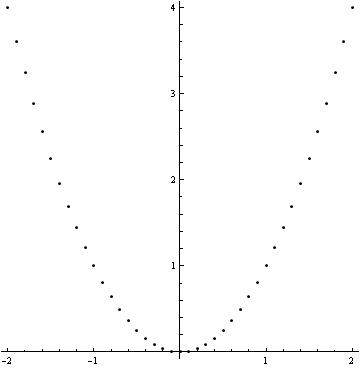
\includegraphics[scale=0.5]{xquadrado-pontos.PNG}
		\caption{Alguns valores de $f(x)=x^2$, $f\colon \mathbb{R}\to\mathbb{R}$}
	\label{fig:xquadrado-pontos}
\end{figure}
Essa função não satisfaz várias propriedades que são "desejáveis", isso é: Ela não é injetora, não é sobrejetora, não é monótona. Vamos tentar melhorar as coisas, restringindo o contra-domínio da nossa função para os reais positivos, de forma que ela se torne sobrejetora. Também podemos restringir nosso domínio de forma que a nova função seja também injetora e monótona. Marcando alguns pontos para essa nova função, obtemos:

\begin{figure}[h]
	\centering
		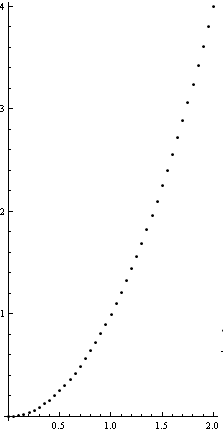
\includegraphics[scale=0.5]{xquadrado-restrita.PNG}
		\caption{Alguns valores de $f(x)=x^2$, $f\colon \mathbb{R}^+ \to \mathbb{R}^+$}
	\label{fig:xquadrado-restrita}
\end{figure}

Vamos agora provar as propriedades que desejamos: Primeiro, se $x<y$ queremos provar que $x^2<y^2$ (lembrando que agora estamos nos restringindo aos números positivos). 

Como $x<y$ então $1<\frac{y}{x}$. Logo $x< y . \frac{y}{x}$ e então $ x^2 < y^2$. Isso prova que a nossa função é monótona, o que garante que ela também é injetora. Podemos imaginar então que o gráfico da função $f(x)=x^2$ é como abaixo:

\begin{figure}[h]
	\centering
		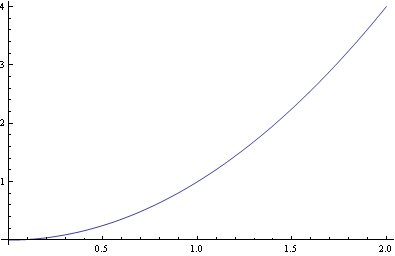
\includegraphics[scale=0.5]{xquadrado-positiva.PNG}
		\caption{Gráfico de $f(x)=x^2$, $f\colon \mathbb{R}^+ \to \mathbb{R}^+$}
	\label{fig:xquadrado-positiva}
\end{figure}

Vamos agora realizar um estudo semelhante, mas como a função $f(x)=x^3$. Alguns valores dessa função são: $1^3=1$, $2^3=8$, $3^3=27$ e assim por diante. Marcando alguns pontos nos eixos cartesianos obtemos a seguinte figura

\begin{figure}[h]
	\centering
		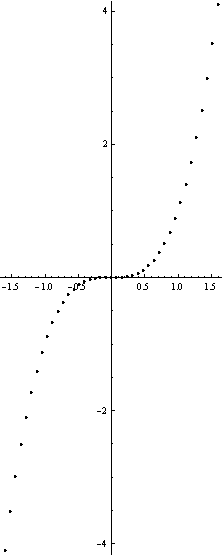
\includegraphics[scale=0.5]{xcubo-pontos.PNG}
		\caption{Gráfico de $f(x)=x^3$, $f\colon \mathbb{R} \to \mathbb{R}$}
	\label{fig:xcubo-pontos}
\end{figure}

Logo percebemos que essa função é extremamente diferente da anterior. Imediatamente temos a sobrejetividade, injetividade e monotocidade, sem nem precisarmos restringir domínio ou contradomínio. Uma demonstração desses fatos pode ser dada por: $$x< y \Rightarrow x^2 < y^2 \text{ e como } x^2>0 \text{ temos } 1 < \frac{y^2}{x^2} \text{ de onde obtemos } x < y . \frac{y^2}{x^2} \text{ assim } x^3 < y^3$$Note que não precisamos supor nada sobre $x$ ou $y$. Como $x^3$ é estritamente crescente, é também injetora.

O gráfico de $f(x) = x^3$ ficaria então:
\begin{figure}[h]
	\centering
		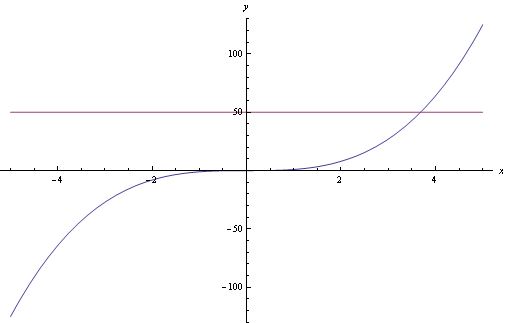
\includegraphics[scale=0.5]{xcubo.PNG}
		\caption{Gráfico de $f(x)=x^3$, $f\colon \mathbb{R} \to \mathbb{R}$}
	\label{fig:xcubo}
\end{figure}

\subsection{Raízes Quadradas e Raízes n-ésimas}
Existem dois tipos de equações que podem surgir envolvendo potenciação. O primeiro, que trataremos agora, é quando a nossa base não muda: por exemplo, como encontrar o número que multiplicado por ele mesmo é igual a 9? Responder a essa pergunta equivale a resolver a seguinte equação: $$x^2=9$$Se tentarmos alguns números, vemos que $x=3$ é uma resposta possível. Mas uma busca mais profunda nos revela que $x=-3$ também é uma resposta possível.

Nesse ponto as coisas começam a ficar diferente da multiplicação por dois motivos: Primeiro, nós encontramos a resposta por tentativa e erro e não seguindo um algoritmo (como o algoritmo da divisão). Segundo, nós encontramos \textit{duas} respostas e não somente uma.

Para piorar a situação: suponha que nós queremos encontrar o número que elevado a segunda potência seja igual a 2, ou, em linguagem simbólica: $$x^2 = 2$$Se nós tentarmos alguns valores vemos que $1^2 = 1.1 = 1$, $2^2 = 2.2 = 4$. Isso é, $1^2$ é menor que $2$, mas $2^2$ é maior que $2$. Isso nos indica que o nosso procurado $x$ está entre $1$ e $2$. Vamos então tentar $x=1,5$ Nesse caso $x^2 = 1,5.1,5 = 2,25$. Assim a raiz da nossa equação é menor do que $1,5$. Podemos tentar $x = 1.4$ e nesse caso obteríamos $x^2 = 1.96$, que é uma boa aproximação, mas não o valor que procurávamos. O que nós sabemos é que a raiz que procuramos está entre $1,4$ e $1,5$ e que poderíamos encontrar uma aproximação tão boa quanto quisermos da raiz da nossa equação.

Um fato chocante, porém, é que a raiz da nossa equação \textit{não} é um número racional. Antes de provar esse fato e todas as complicações que surgem do mesmo, vamos adotar uma notação, chamaremos a raiz de nossa equação que está entre $1,4$ e $1,5$ de  $\sqrt{2}$. 
